    \documentclass[dvipsnames]{beamer}
    \usetheme{Madrid}
    \usefonttheme{professionalfonts}
    \usepackage{
        amsmath,
        amssymb,
        fouriernc, % fourier font w/ new century book
        fancyhdr, % page styling
        lastpage, % footer fanciness
        hyperref, % various links
        setspace, % line spacing
        amsthm, % newtheorem and proof environment
        mathtools, % \Aboxed for boxing inside aligns, among others
        float, % Allow [H] figure env alignment
        enumerate, % Allow custom enumerate numbering
        graphicx, % allow includegraphics with more filetypes
        wasysym, % \smiley!
        upgreek, % \upmu for \mum macro
        listings, % writing TrueType fonts and including code prettily
        tikz, % drawing things
        booktabs, % \bottomrule instead of hline apparently
        cancel % can cancel things out!
    }
    \usepackage[
        labelfont=bf, % caption names are labeled in bold
        font=scriptsize % smaller font for captions
    ]{caption}
    \usepackage[font=scriptsize]{subcaption} % subfigures

    \newcommand*{\scinot}[2]{#1\times10^{#2}}
    \newcommand*{\dotp}[2]{\left<#1\,\middle|\,#2\right>}
    \newcommand*{\rd}[2]{\frac{\mathrm{d}#1}{\mathrm{d}#2}}
    \newcommand*{\pd}[2]{\frac{\partial#1}{\partial#2}}
    \newcommand*{\rtd}[2]{\frac{\mathrm{d}^2#1}{\mathrm{d}#2^2}}
    \newcommand*{\ptd}[2]{\frac{\partial^2 #1}{\partial#2^2}}
    \newcommand*{\md}[2]{\frac{\mathrm{D}#1}{\mathrm{D}#2}}
    \newcommand*{\pvec}[1]{\vec{#1}^{\,\prime}}
    \newcommand*{\svec}[1]{\vec{#1}\;\!}
    \newcommand*{\bm}[1]{\boldsymbol{\mathbf{#1}}}
    \newcommand*{\ang}[0]{\;\text{\AA}}
    \newcommand*{\mum}[0]{\\;upmu \mathrm{m}}
    \newcommand*{\at}[1]{\left.#1\right|}

    \let\Re\undefined
    \let\Im\undefined
    \DeclareMathOperator{\Res}{Res}
    \DeclareMathOperator{\Re}{Re}
    \DeclareMathOperator{\Im}{Im}
    \DeclareMathOperator{\Log}{Log}
    \DeclareMathOperator{\Arg}{Arg}
    \DeclareMathOperator{\Tr}{Tr}
    \DeclareMathOperator{\E}{E}
    \DeclareMathOperator{\Var}{Var}
    \DeclareMathOperator*{\argmin}{argmin}
    \DeclareMathOperator*{\argmax}{argmax}
    \DeclareMathOperator{\sgn}{sgn}
    \DeclareMathOperator{\diag}{diag\;}

    \DeclarePairedDelimiter\bra{\langle}{\rvert}
    \DeclarePairedDelimiter\ket{\lvert}{\rangle}
    \DeclarePairedDelimiter\abs{\lvert}{\rvert}
    \DeclarePairedDelimiter\ev{\langle}{\rangle}
    \DeclarePairedDelimiter\p{\lparen}{\rparen}
    \DeclarePairedDelimiter\s{\lbrack}{\rbrack}
    \DeclarePairedDelimiter\z{\lbrace}{\rbrace}

    % \everymath{\displaystyle} % biggify limits of inline sums and integrals
    \tikzstyle{circ} % usage: \node[circ, placement] (label) {text};
        = [draw, circle, fill=white, node distance=3cm, minimum height=2em]
    \definecolor{commentgreen}{rgb}{0,0.6,0}
    \lstset{
        basicstyle=\ttfamily\footnotesize,
        frame=single,
        numbers=left,
        showstringspaces=false,
        keywordstyle=\color{blue},
        stringstyle=\color{purple},
        commentstyle=\color{commentgreen},
        morecomment=[l][\color{magenta}]{\#}
    }

\begin{document}

\title{Critical Layer Absorption and Tidal Spin-Up}
\subtitle{Group Meeting}
\author{Yubo Su}
\date{Sept 21, 2018}

\maketitle

\begin{frame}
    \frametitle{Background}
    \framesubtitle{Goldreich \& Nicholson 1989}

    \begin{itemize}
        \item \emph{Tidal Friction in Early-Type Stars}.

        \item Tidal torques excite outgoing internal gravity waves (IGW) at
            boundary between convective core and radiative envelope.

        \item IGW amplify as they propagate due to density rarefaction.

        \item Dissipate in the envelope to mean flow,

        \item Transfers energy from the orbit to the star and synchronizing the
            spin to the orbit outside-in.
    \end{itemize}
    \begin{figure}[t]
        \centering
        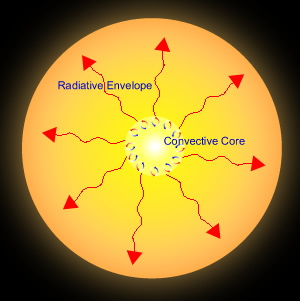
\includegraphics[width=0.3\textwidth]{conv_core.jpg}
    \end{figure}
\end{frame}

\begin{frame}
    \frametitle{Background}
    \framesubtitle{Barker \& Ogilvie 2010}

    \begin{itemize}
        \item Barker \& Ogilvie 2010 present a similar picture for solar-type
            stars (radiative core and convective envelope).
            \begin{figure}[h]
                \centering
                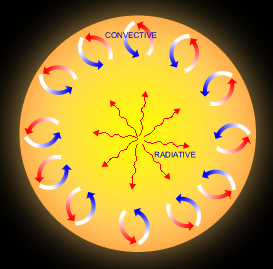
\includegraphics[width=0.3\textwidth]{rad_core.jpg}
            \end{figure}

        \item IGW propagate inwards instead, ampliffying via geometric focusing,
            and spin up the star inside-out.

        \begin{itemize}
            \item Perform 2D simulations.
            \item Observe two phases of spin-up: mean flow formation, corotation
                absorption (mean flow corotates with companion).
        \end{itemize}
    \end{itemize}
\end{frame}

\begin{frame}
    \frametitle{Background}
    \framesubtitle{Plane Parallel Papers of Critical Layers
        (Atmospheric Sciences)}
    \begin{itemize}
        \item Linear, inviscid theory of critical layers predicts almost
            complete absorption (Booker \& Bretherton 1967). Viscosity same
            (Hazel 1967).

        \item Weakly nonlinear theory predicts reflection! Predicts reflection
            appears after $\mathcal{O}\p*{A^{-2/3}}$ (Brown \& Stewartson 1980).

        \item 3D plane-parallel simulation shows reflection at nonzero amplitude
            (Winters \& d'Asaro 1994).

        \item \textbf{Question: What happens in other geometries?}
    \end{itemize}
\end{frame}

\begin{frame}
    \frametitle{Work}
    \framesubtitle{2D Plane Parallel Case}

    \begin{itemize}
        \item Begin with incompressible fluid equations in the presence of
            stratification $\rho_0 \propto e^{-z/H}$ and shear flow $\vec{u}_0 =
            u_0(z)\hat{x}$:
            \begin{subequations}
                \begin{align}
                    \vec{\nabla} \cdot \vec{u}_1 &= 0,\\
                    \pd{\rho_1}{t} + \p*{\vec{u} \cdot \vec{\nabla}}\rho_1
                        - u_{1z}\frac{\rho_0}{H} &= 0,\\
                    \pd{u_{1x}}{t} + \p*{\vec{u} \cdot \vec{\nabla}}\p*{u_{1x} +
                        u_0} + \frac{1}{\rho_0}\pd{P}{x} &= 0,\\
                    \pd{u_{1z}}{t} + \p*{\vec{u} \cdot \vec{\nabla}}u_{1z} +
                        \frac{1}{\rho_0}\pd{P}{z} + \frac{\rho_1 g}{\rho_0} &= 0.
                \end{align}
            \end{subequations}

        \item Linearize and math ($\omega_{cr} = \omega - k_xu_0$)
            \begin{equation}
                \ptd{u_{1z}}{z} - \frac{1}{H}\pd{u_{1z}}{z} + \s*{
                    \frac{k_x^2N^2}{\omega_{cr}^2}
                        - k_x^2
                        - \frac{k_x}{\omega_{cr}H}\pd{u_0}{z}
                        + \frac{k_x}{\omega_{cr}} \ptd{u_0}{z}
                } u_{1z} = 0. \label{eq:shear_lin_uz}
            \end{equation}
    \end{itemize}
\end{frame}

\begin{frame}
    \frametitle{Work}
    \framesubtitle{2D Plane Parallel Case}

    \begin{itemize}
        \item Near critical layer, $\ptd{u_{1z}}{z} +
            \frac{k_x^2N^2}{\omega_{cr}^2}u_{1z} = 0$, $\omega_{cr} \propto k_x
            \pd{u_0}{z}\delta z$ where $\delta z = z - z_c$ is distance to
            critical layer.

        \item Power series ansatz, $u_{1z} \propto \omega_{cr}^\alpha \propto
            (\delta z)^{\alpha}$ gives
            \begin{equation}
                \alpha = \frac{1}{2}\pm i\sqrt{\frac{N^2}{\p*{\pd{u_0}{z}}^2} -
                    \frac{1}{4}} = \frac{1}{2}
                        \pm i\sqrt{\mathrm{Ri} - \frac{1}{4}}.
            \end{equation}

        \item Move $\omega_{cr} \to \omega_{cr} + i\omega_i$ (growing
            perturbation), specify branch cuts for $u_{1z}$!

        \begin{figure}[t]
            \centering
            \begin{tikzpicture}
                \draw[->] (0, 0) -- (0, 1);
                \draw[<->] (-3, 0) -- (3, 0);
                \filldraw[black] (0, 1.1) circle(0.05);
                \filldraw[black] (0, 0) circle(0.05);
                \node[above right] at (0, 0) {$\omega_{cr}$};
                \node[above right] at (0, 1) {$\omega_{cr} + i\omega_i$};
                \node[above right] at (3, 0) {$\mathbb{R}$};
            \end{tikzpicture}
        \end{figure}
    \end{itemize}
\end{frame}

\begin{frame}
    \frametitle{Work}
    \framesubtitle{2D Plane Parallel Case}

    \begin{itemize}
        \item Call being above the critical layer $\Arg(\delta z) = 0$, then
            below the critical layer $\Arg(\delta z) = -\pi$. This gives
            \begin{equation}
                \p*{\delta z}^{\frac{1}{2} \pm i\mu} =
                    \begin{cases}
                        \abs*{\delta z}^{\frac{1}{2}\pm i\mu}
                          & \Re \delta z > 0,\\
                        \abs*{\delta z}^{\frac{1}{2}\pm i\mu}
                            e^{-\frac{i\pi}{2}}e^{\mp \mu \pi} & \Re \delta z <
                            0.
                    \end{cases}
            \end{equation}

        \begin{itemize}
            \item Why specify above? Physically we know only one type of wave
                above, should have less complexity after branch cut, Papers
                don't elaborate, I think inspired guess.
        \end{itemize}

        \item $\abs*{\delta z}^{\pm i\mu} = e^{\pm i\mu \ln \abs*{\delta z}}$,
            liberally interpret $\sim e^{\pm ik_z \abs*{\delta z}}$.

        \item If so, $e^{-ik_z \delta z}e^{+\mu \pi}, e^{+ik_z \delta z}e^{-\mu
            \pi}$. But for IGW, $k_z < 0$ means \emph{upward-propagating}!
    \end{itemize}
\end{frame}

\begin{frame}
    \frametitle{Work}
    \framesubtitle{2D Plane Parallel Conclusion}

    \begin{figure}[t]
        \centering
        \begin{tikzpicture}
            \node (center) {};
            \node[above left of = center] (in) {};
            \node[above left of = in] (in2)
                {$e^{-ik_z \delta z} e^{+\mu \pi}$};
            \node[below left of = center] (out) {};
            \node[below left of = out] (out2)
                {$e^{+ik_z \delta z} e^{-\mu \pi}$};
            \node[right of = center] (trans) {};
            \node[right of = trans] (trans2) {$1$};
            \draw[->] (in2) -- (center);
            \draw[->] (center) -- (out2);
            \draw[->] (center) -- (trans2);
        \end{tikzpicture}
    \end{figure}
\end{frame}

\end{document}
